\begin{frame}{Interpolation vs. Extrapolation with Convex Hull \cite{balestriero2021learninghighdimensionamounts} \cite{boyd2004convex}}
     \label{def7}
    Given a model $\hat f$ trained on a set of points $\mathcal X^{\text{tr}}$, the convex hull of $\mathcal X^{\text{tr}}$, denoted as $\text{Conv}\left(\mathcal X^{\text{tr}}\right)$.
    For any point $\mathbf x \sim \mathcal X^{\text{te}}$ and $\mathcal X^{\text{te}} \cap \mathcal X^{\text{tr}} = \emptyset$:
    \begin{itemize}
        \item Interpolation occurs when $\mathbf x \in \text{Conv}\left(\mathcal X^{\text{tr}}\right)$.
        \item Extrapolation occurs when $\mathbf x \notin \text{Conv}\left(\mathcal X^{\text{tr}}\right)$.
    \end{itemize}

    \begin{figure}[H]
    \centering
    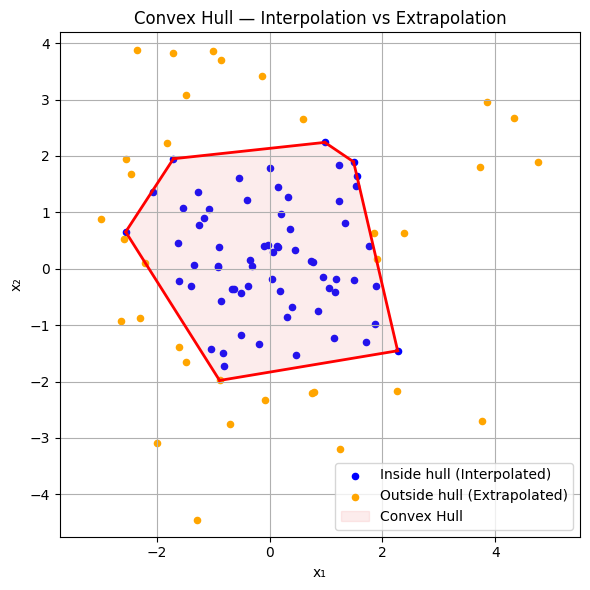
\includegraphics[width=0.5\textwidth]{figures/fig_2.png}
    \label{fig:fig_2}
\end{figure}
\end{frame}